\documentclass[]{article}
\usepackage{amsmath, amsfonts, amssymb, dsfont}
\usepackage{float}
\usepackage{fancyhdr}
\usepackage{fontawesome5}
\usepackage{mathrsfs}
\usepackage{amsmath}
\allowdisplaybreaks 

\usepackage{tikz}
\usetikzlibrary{automata, positioning}
\usepackage{placeins}
\usepackage{diagbox}
\usepackage[utf8]{inputenc}


\usepackage{graphicx, adjustbox, float, xcolor}


\usepackage{tikz, pgfplots}
\pgfplotsset{compat=1.17}

\usetikzlibrary{arrows.meta, automata, positioning, decorations.pathreplacing, decorations.markings}
\newcommand{\interior}[1]{%
  {\kern0pt#1}^{\mathrm{o}}%
}


\usepackage{booktabs, enumitem, caption}


\usepackage{minted}
\usemintedstyle{friendly}
\setminted{fontsize=\small,autogobble,mathescape}

\usepackage[a4paper,
  includehead,includefoot,
  top=5mm,            
  headheight=15pt,    
  headsep=1pt,        
  bottom=20mm,left=40mm,right=40mm
]{geometry}

\pagestyle{fancy}


\lhead{Ben Vickers - 304024}
\rhead{Numerical Analysis Project - Solving Non-Linear Ordinary Differential Equations in Practice}
\setlength{\headsep}{0.4cm}
\usepackage{titling}
\setlength{\droptitle}{-70pt}   

\title{\textbf{Numerical Analysis Project - Solving Non-Linear Ordinary Differential Equations in Practice}}
\author{Ben Vickers - 304024}
\date{\textbf{Due: 13:59, Thursday 11 December 2025}}

\begin{document}

	\maketitle

\section*{Solving non-linear ordinary differential equations in practice}

\noindent Consider the function $\psi : (-1,1) \to \mathbb{R}$ given by
\[
\psi(s)
= \frac{\theta}{2}\left( (1+s)\log\left(\frac{1+s}{2}\right)
+ (1-s)\log\left(\frac{1-s}{2}\right) \right) - (s^{2}-1),
\]
where $\theta > 0$ is a positive parameter. The derivative is given by
\[
\psi'(s) = \frac{\theta}{2}\left(\log(1+s) - \log(1-s)\right) - 2s.
\]

\noindent Consider the ODE
\[
\dot{y} = -\psi'(y), \qquad y(0) = y_0
\]
for some $y_0 \in (-1,1)$.
\begin{enumerate}
  \item The limit $\theta \to 0$ is known as the \emph{deep quench limit}. Plot $\psi$ on $(-1,1)$ for the choices of $\theta \in \{8,4,2,1\}$.
\end{enumerate}

\noindent \textbf{SOLUTION:} \newline

\noindent Using Python, we obtain the following plot of $\psi$ on $(-1,1)$ for the choices of $\theta \in \{8,4,2,1\}$

\begin{figure}[!htb]
    \centering
    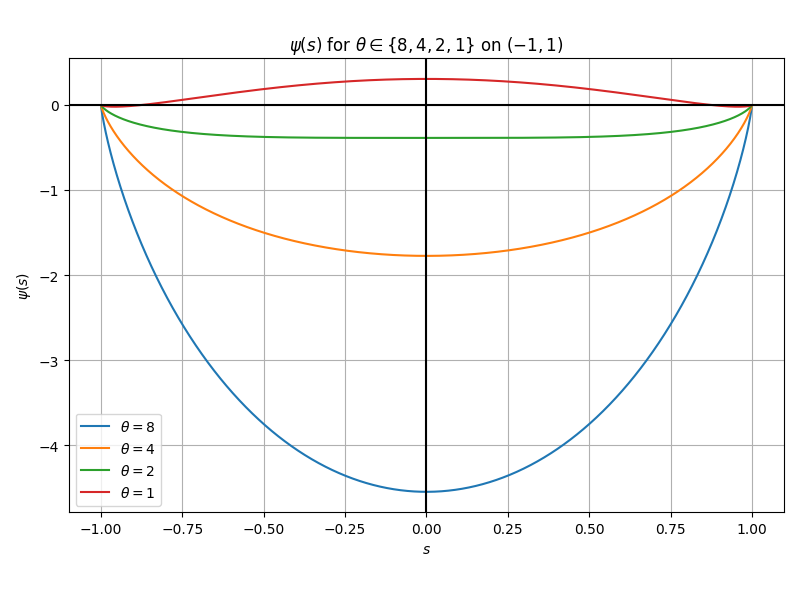
\includegraphics[width=1\linewidth]{Project plots/phi.png}
    \vspace{-1cm}
    \caption{$\psi(s)$ for $\theta \in \{8,4,2,1\}$ on $(-1,1)$}
\end{figure}\FloatBarrier
\newpage
\begin{enumerate}
    \setcounter{enumi}{1}
  \item For the same choices of $\theta$, plot $\psi'$ on $(-1,1)$.
  \end{enumerate}
  \noindent \textbf{SOLUTION:} \newline

\noindent Using Python, we obtain the following plot of $\psi'$ on $(-1,1)$ for the same choices of $\theta \in \{8,4,2,1\}$

\begin{figure}[!htb]
    \centering
    \vspace{-0.4cm}
    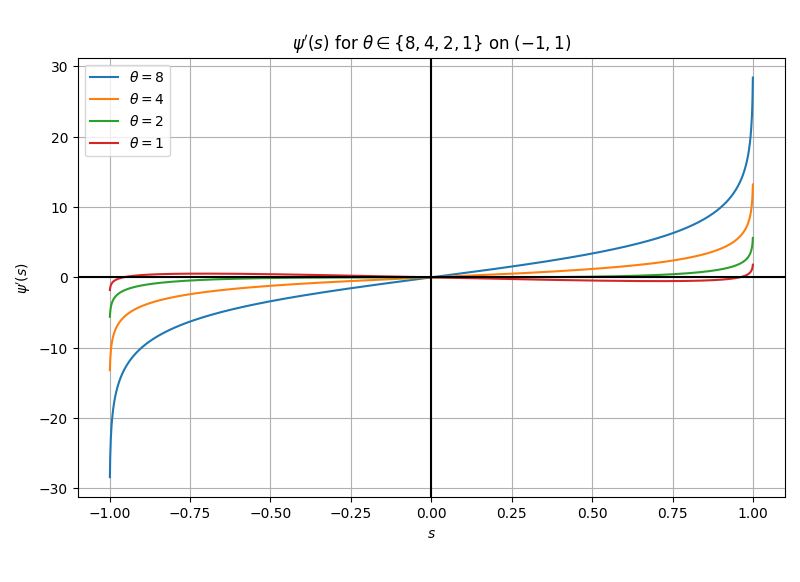
\includegraphics[width=1\linewidth]{Project plots/phiprime.png}
    \vspace{-1.2cm}
    \caption{$\psi'(s)$ for $\theta \in \{8,4,2,1\}$ on $(-1,1)$}
\end{figure}\FloatBarrier
\begin{enumerate}
    \setcounter{enumi}{2}
    \vspace{-0.4cm}
  \item Show that there exists a unique solution to the ODE for at least a small time. It is important to use that $y_0 \in (-1,1)$.
  \end{enumerate}
  \noindent \textbf{SOLUTION:} \newline

  \noindent We can define \vspace{-0.2cm} \[ 
  f(t,y) := -\psi'(y) = -\frac{\theta}{2}\left(\log(1+y) - \log(1-y)\right) + 2y
  \] 
 Where $\log$ denotes the natural log. Then we have the IVP:
  \[
  \dot{y} = f(t,y), \qquad y(0) = y_0 \in (-1,1)
  \]
  \noindent We aim to apply the Picard–Lindelöf theorem (Theorem 5.8) which gives us that there exists a unique solution to the ODE for at least a small time.\newline

\noindent We can firstly observe that $\psi'$ is continuous (only) on $(-1,1)$ since its logarithm terms are defined only for $1\pm y > 0 \iff y\in (-1,1)$. Hence $f = -\psi'$ is continuous on $(-1,1)$. (see Figure 5 for plot of $f$ on $y \in (-1,1)$.)\newline

    \noindent Since we have $y_0 \in (-1,1)$ (which importantly is open), we can choose $r\in(0,1): r\in (|y_0|,1) \implies [-r,r] \subset (-1,1)$. Then we can define the interval $I := [0,T]$ for some $T >0$ and the domain $D:=I \times [-r,r] \subset \mathbb{R} \times \mathbb{R}$. Then we have that $(0,y_0)\in \interior{D}$ for any $y_0 \in (-1,1)$. Hence because $[-r,r] \subset (-1,1)$, $f$ will be continuous on its entire domain, $D$ and therefore also around a neighbourhood of $(0,y_0)$.\newline

    \noindent  Now we need to check that $f$ is Lipschitz in $y$ around $(0,y_0)$. We have:\newline
    \begin{align*}
    |f(t,y_1)-f(t,y_2)| &= \left| -\frac{\theta}{2}\left(\log(1+y_1) - \log(1-y_1)\right) + \frac{\theta}{2}\left(\log(1+y_2) - \log(1-y_2)\right) + 2(y_1-y_2) \right|\\
    &\leq \dfrac{\theta}{2} \left| \left[ \log(1+y_2)-\log(1-y_2)\right] - \left[ \log(1+y_1)-\log(1-y_1)\right] \right| + 2|y_1-y_2|
    \end{align*}
   We can now define:
    \[
    \ell : (-1,1) \to \mathbb{R}\,,\, \ell(x) :=\log(1+x)-\log(1-x) 
    \]
     \begin{align*}
   \implies  |f(t,y_1)-f(t,y_2)| &\leq  \dfrac{\theta}{2} \left| \left[ \log(1+y_2)-\log(1-y_2)\right] - \left[ \log(1+y_1)-\log(1-y_1)\right] \right| + 2|y_1-y_2|\\
   &= \dfrac{\theta}{2} \left| \ell(y_2) - \ell(y_1)\right| + 2|y_1-y_2|
    \end{align*}
\noindent Since $\ell$ is $C^1$ on $(-1,1)$, then $\forall y_1,y_2 \in [-r,r]$, (where we recall $r\in(0,1)$), we have by MVT, $\exists \tilde{y} \in (\min\{y_1,y_2\}, \max\{y_1,y_2\}), \text{ (i.e. between $y_1$ and $y_2$!)  such that}:$
\begin{align*}
\ell(y_1)-\ell(y_2) &= \ell'(\tilde{y})(y_1-y_2)\\
\implies \left| \ell(y_1)-\ell(y_2)\right| &\leq \sup_{\tilde{y} \in [-r,r]} |\ell'(\tilde{y})||y_1-y_2|\\
&= \sup_{\tilde{y} \in [-r,r]} \left|\left[ \frac{1}{1+\tilde{y}} + \frac{1}{1-\tilde{y}}\right]\ \right||y_1-y_2|\\
&= \sup_{\tilde{y} \in [-r,r]} \left|\left[ \frac{2}{1-\tilde{y}^2}\right] \right||y_1-y_2|\\
&=  \frac{2}{1-r^2} |y_1-y_2|\\
   \implies  |f(t,y_1)-f(t,y_2)| &\leq \dfrac{\theta}{2} \left| \ell(y_2) - \ell(y_1)\right| + 2|y_1-y_2|\\
   &\leq  \frac{\theta}{2}\cdot \frac{2}{1-r^2} |y_1-y_2| + 2|y_1-y_2|\\
   &= \left(\frac{\theta}{1-r^2}+2\right)|y_1-y_2|
    \end{align*}
Hence we can define:
\[
K_{\theta} :=\frac{\theta}{1-r^2}+2 \qquad =\text{ the Lipschitz constant of $f$ given $\theta$.}
\]
    Then $\forall t \in [0,T]$ and $y_1,y_2 \in [-r,r]$ we have:
 \[
  |f(t,y_1)-f(t,y_2)| \leq K_\theta |y_1 - y_2|
\]
Therefore $f$ is indeed Lipschitz in its second variable on its domain  $D := [0,T] \times [-r,r]$. \newline

\noindent Therefore applying Theorem 5.8, it holds that $\exists \delta > 0$ such that a unique solution to the IVP, $Y(t)$ exists on $[0,\delta]$ (i.e. for a `small' time), where $Y(0) = y_0$.

\begin{enumerate}
    \setcounter{enumi}{3}
  \item Now consider $\theta = 1$. For each of the timesteps $\delta t \in \{0.1,0.05,0.025,0.0125\}$, use the explicit Euler method to numerically solve the ODE until time $T = 1$. This should be done for each of the three initial conditions $y_0 = -0.5$, $y_0 = 0$, and $y_0 = 0.5$.
  \end{enumerate}


  \noindent \textbf{SOLUTION:} \newline

    \noindent If we have that $\theta = 1$, then we have:
    \[
    f(t,y) = -\frac{1}{2}\left(\log(1+y) - \log(1-y)\right) + 2y
    \]
    \noindent Given each $\delta t > 0$, if we want to solve the ODE until $T=1$ then we have:
    \[
    t_n = n \delta t, \qquad n=0,1,\dots , \dfrac{T}{\delta t} =  \dfrac{1}{\delta t}
    \]
    \noindent Whereby the obtained values of $y^n$ approximate $Y(t_n)$ where $Y$ is the solution to the given IVP. Now we can apply the forward Euler scheme for each of the timesteps $\delta t \in \{0.1,0.05,0.025,0.0125\}$ and for each of the three initial conditions $y_0 = -0.5$, $y_0 = 0$, and $y_0 = 0.5$. (The code used to obtain $y^{\dfrac{1}{\delta t}} \approx Y(1)$ for each initial condition is given in Appendix A)\newline   
        \begin{enumerate}
      \item For $y_0 = -0.5$:
      \begin{itemize}
        \item For $\delta t = 0.1$:
        \begin{align*}
        y^0 &= y_0 = -0.5\\
        y^1 &= y^0 + 0.1f(y^0) = -0.5+0.1\cdot f(-0.5) = -0.5+0.1\cdot -0.45069 = -0.545069\\
             & \smash{\vdots} \\
        y^{10} &= -0.95009359 \approx Y(t_{10}) = Y(1)
        \end{align*}
        
    \item For $\delta t = 0.05$:
        \begin{align*}
        y^0 &= y_0 = -0.5\\
        y^1 &= y^0 + 0.05f(y^0) = -0.5+0.05\cdot f(-0.5) = -0.5+0.05\cdot -0.45069 = -0.5225345\\
             & \smash{\vdots} \\
        y^{20} &= -0.94495140   \approx Y(t_{20}) = Y(1)
        \end{align*}

    \item For $\delta t = 0.025$:
        \begin{align*}
        y^0 &= y_0 = -0.5\\
        y^1 &= y^0 + 0.025f(y^0) = -0.5+0.025\cdot f(-0.5) = -0.5+0.025\cdot -0.45069 = -0.51126725\\
             & \smash{\vdots} \\
        y^{40} &= -0.94270604 \approx Y(t_{40}) = Y(1)
        \end{align*}

    \item For $\delta t = 0.0125$:
        \begin{align*}
        y^0 &= y_0 = -0.5\\
        y^1 &= y^0 + 0.0125f(y^0) = -0.5+0.0125\cdot f(-0.5) = -0.5+0.0125\cdot -0.45069 = -0.505633625\\
             & \smash{\vdots} \\
        y^{80} &= -0.94163941  \approx Y(t_{80}) = Y(1)
        \end{align*}
      \end{itemize}

\item For $y_0 = 0$:
      \begin{itemize}
        \item For $\delta t = 0.1$:
        \begin{align*}
        y^0 &= y_0 = 0\\
        y^1 &= y^0 + 0.1f(y^0) = 0+0.1\cdot f(0) = 0+0.1\cdot 0 = 0\\
      & \smash{\vdots} \\
        y^{10} &= 0  \approx Y(t_{10}) = Y(1)
        \end{align*}
        
    \item For $\delta t = 0.05$:
        \begin{align*}
        y^0 &= y_0 = 0\\
        y^1 &= y^0 + 0.05f(y^0) = 0+0.05\cdot f(0) = 0+0.05\cdot 0 = 0\\
      & \smash{\vdots} \\
        y^{20} &= 0 \approx Y(t_{20}) = Y(1)
        \end{align*}

    \item For $\delta t = 0.025$:
        \begin{align*}
        y^0 &= y_0 = 0\\
        y^1 &= y^0 + 0.025f(y^0) = 0+0.025\cdot f(0) = 0+0.025\cdot 0 = 0\\
      & \smash{\vdots} \\
        y^{40} &= 0 \approx Y(t_{40}) = Y(1)
        \end{align*}

    \item For $\delta t = 0.0125$:
       \begin{align*}
        y^0 &= y_0 = 0\\
        y^1 &= y^0 + 0.0125f(y^0) = 0+0.0125\cdot f(0) = 0+0.0125\cdot 0 = 0\\
      & \smash{\vdots} \\
        y^{80} &= 0 \approx Y(t_{80}) = Y(1)
        \end{align*}
\end{itemize}

 \item For $y_0 = 0.5$:
      \begin{itemize}
        \item For $\delta t = 0.1$:
        \begin{align*}
        y^0 &= y_0 = 0.5\\
        y^1 &= y^0 + 0.1f(y^0) = 0.5+0.1\cdot f(0.5) = 0.5+0.1\cdot 0.45069 = 0.545069\\
      & \smash{\vdots} \\
        y^{10} &= 0.95009359 \approx Y(t_{10}) = Y(1)
        \end{align*}
        
    \item For $\delta t = 0.05$:
        \begin{align*}
        y^0 &= y_0 = 0.5\\
        y^1 &= y^0 + 0.05f(y^0) = 0.5+0.05\cdot f(0.5) = 0.5+0.05\cdot 0.45069 = 0.5225345\\
      & \smash{\vdots} \\
        y^{20} &= 0.94495140 \approx Y(t_{20}) = Y(1)
        \end{align*}

    \item For $\delta t = 0.025$:
        \begin{align*}
        y^0 &= y_0 = 0.5\\
        y^1 &= y^0 + 0.025f(y^0) = 0.5+0.025\cdot f(0.5) = 0.5+0.025\cdot 0.45069 = 0.51126725\\
      & \smash{\vdots} \\
        y^{40} &= 0.94270604  \approx Y(t_{40}) = Y(1)
        \end{align*}

    \item For $\delta t = 0.0125$:
        \begin{align*}
        y^0 &= y_0 = 0.5\\
        y^1 &= y^0 + 0.0125f(y^0) = 0.5+0.0125\cdot f(0.5) = 0.5+0.0125\cdot 0.45069 = 0.505633625\\
      & \smash{\vdots} \\
        y^{80} &= 0.94163941  \approx Y(t_{80}) = Y(1)
        \end{align*}
      \end{itemize}
    \end{enumerate}

\noindent Tabulating these results to have an easier visualisation of the results gives Table 1:
\begin{table}[H]
  \centering
  \caption{Forward Euler solutions of IVP at $T=1$ for $y_0 \in \{-0.5, \,0,\,0.5\}$, and $\delta t \in \{0.1,0.05,0.025,0.0125\}$}
  \begin{tabular}{c|cccc}
    \hline
    \diagbox[
      innerwidth=2em,     
      height=2em,        
      innerleftsep=0.8em, 
      innerrightsep=0.8em 
    ]{$y_0$}{$\delta t$}
    & $0.1$ & $0.05$ & $0.025$ & $0.0125$ \\
    \hline
    $-0.5$ & $-0.95009359$ & $-0.94495140$ & $-0.94270604$ & $-0.94163941$ \\
    $0$    & $0.00000000$  & $0.00000000$  & $0.00000000$  & $0.00000000$  \\
    $0.5$  & $0.95009359$  & $0.94495140$  & $0.94270604$  & $0.94163941$  \\
    \hline
  \end{tabular}
\end{table}

\begin{enumerate}
    \setcounter{enumi}{4}
  \item Hence determine the value $\displaystyle \lim_{t \to \infty} Y(t)$.
  \end{enumerate}
  
  \noindent \textbf{SOLUTION:} \newline

  
\noindent It seems clear from our results obtained above that $\displaystyle \lim_{t \to \infty} Y(t)$ will depend only on the sign of $y_0$. I.e., $y_0 \mapsto \displaystyle \lim_{t \to \infty} Y(t)$ is piecewise constant.\newline

\noindent To determine the value of $\displaystyle \lim_{t \to \infty} Y(t)$ (still assuming $\theta = 1$) we have that if:
\[\lim_{t \to \infty} Y(t) =: L_{y_0} \in (-1,1),  \implies f(L_{y_0}) = 0. \,\text{ I.e., }  L_{y_0} \text{ is a steady state.} \]
\begin{align*}
  \implies  f(L_{y_0}) =  -\frac{1}{2}\left(\log(1+L_{y_0}) - \log(1-L_{y_0})\right) + 2L_{y_0} &= 0\\
\implies \log(1+L_{y_0}) - \log(1-L_{y_0}) &= 4L_{y_0}\\
\implies \log\left(\dfrac{1+L_{y_0}}{1-L_{y_0}}\right) &= 4L_{y_0} \\
\implies 2 \text{arctanh}(L_{y_0}) &= 4L_{y_0} \\
\implies L_{y_0} &= \text{tanh}(2L_{y_0})
\end{align*}
\vspace{-0.3cm}
\noindent From Figure 3 below we therefore have: $L_{y_0} = 0, \quad L_{y_0} = \pm0.9575$
\begin{figure}[!htb]
    \centering
 \vspace{0.3cm}
    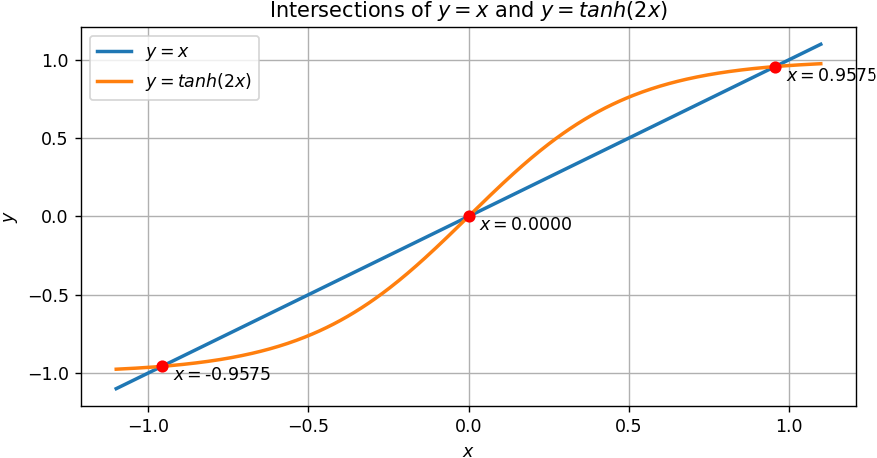
\includegraphics[width=1\linewidth]{Project plots/tanhv4.png}
    \vspace{-0.4cm}
    \caption{Intersections of $y=x$ and $y=\tanh(2x)$}
\end{figure}
  \FloatBarrier
\noindent Where we can then infer from Table 1 obtained by forward Euler that:
\[
\begin{cases}
    L_{y_0} = 0 & \text{ if } y_0 =0\\
    L_{y_0} = -0.9575& \text{ if } y_0 =-0.5\\
        L_{y_0} = 0.9575& \text{ if } y_0 =0.5
\end{cases}
\]
\noindent This can be observed from a phase plane portrait of the IVP in Figure 4:
\vspace{-0.1cm}
\begin{figure}[!htb]
    \centering
    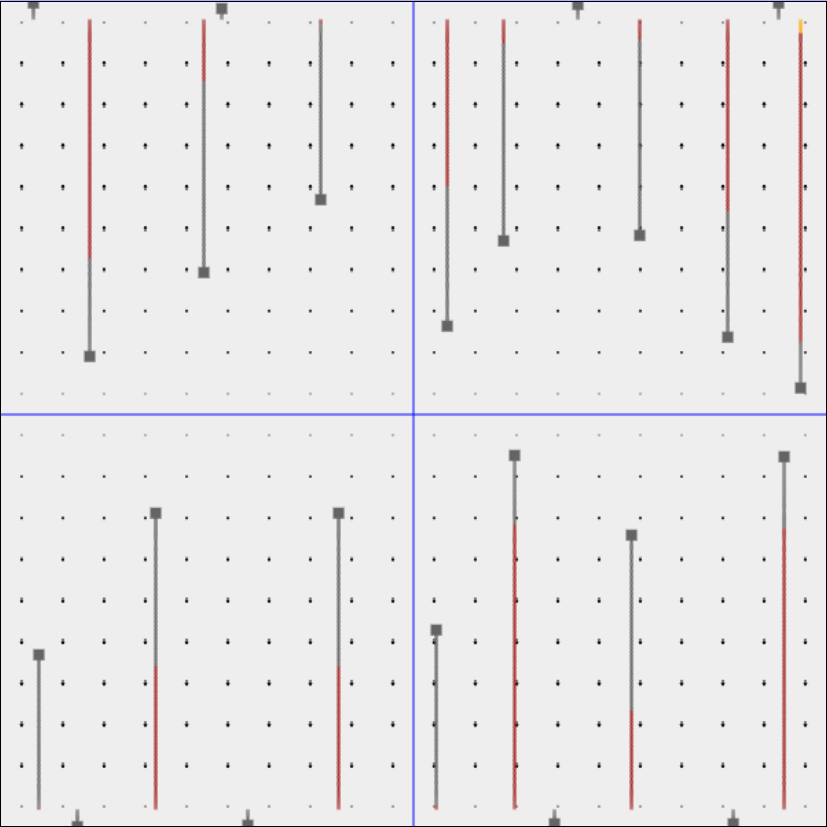
\includegraphics[width=0.82\linewidth]{Project plots/phase plane.png}
    \caption{Phase plane portrait of IVP. $y(0)$ is indicated by grey squares.
    Generated by the phase plane plotter at aeb019.hosted.uark.edu/pplane.html by Ariel Barton}
    IVP: $\displaystyle \begin{cases}
    \dfrac{dx}{dt} & \displaystyle= 0\\[8pt]
\dfrac{dy}{dt} &=  \displaystyle -\dfrac{1}{2}\left(\log(1+y) - \log(1-y)\right) + 2y
\end{cases}$
\end{figure}\FloatBarrier
\newpage
\noindent Figure 4 also shows that the solutions are not dependent on the exact value of $y_0$, rather, only its sign. To formally confirm these results, we can observe the plot of $f(t,y)$ given below in Figure 5:

\begin{figure}[!htb]
    \centering
    \vspace{-0.1cm}
    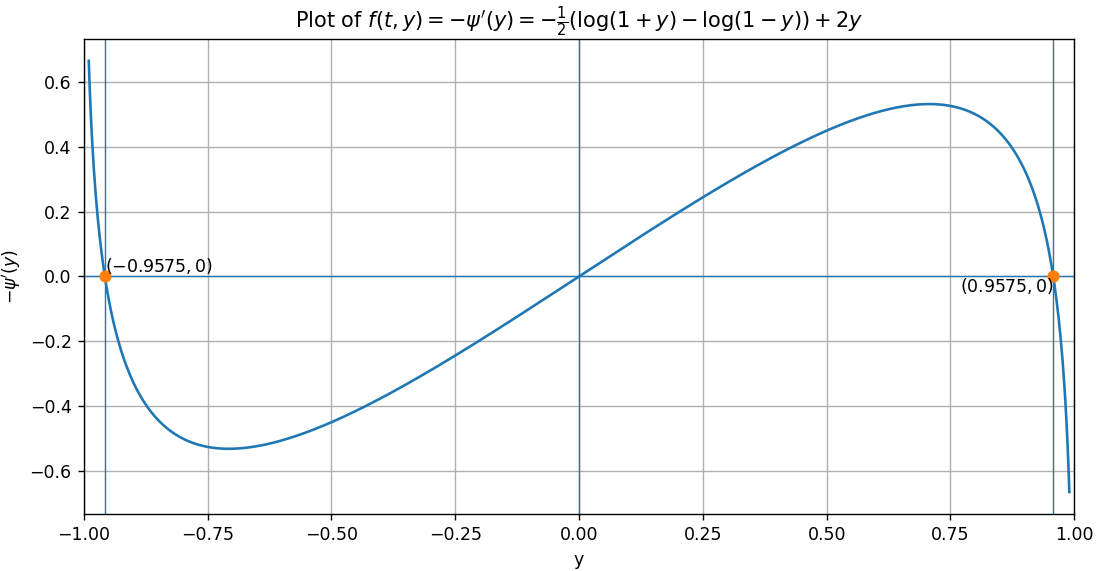
\includegraphics[width=1\linewidth]{Project plots/psiprimev2.png}
    \vspace{-0.4cm}
    \caption{Plot of $f(t,y) = -\psi'(y) = -\frac{1}{2}(\log(1+y)-\log(1-y)) + 2y$}
\end{figure}\FloatBarrier


We see here that $f$ (as we previously noted) is continuous on $(-1,1)$ and:
\begin{itemize}
    \item $f(y)=0$ for only $y \in \{-0.9575,0,0.9575\}$
    \item $f(y)>0$ for all $y \in (0,0.9575)$
    \item $f(y) < 0$ for all $y \in (0.9575,1)$
    \item $f(y) <0$ for all $y \in (-0.9575,0)$
    \item $f(y) > 0$ for all $y \in (-1,-0.9575)$
\end{itemize}

\noindent So what we have is that for each interval of initial conditions:
\begin{enumerate}
    \item If $y_0 = 0$ then $\forall t\geq 0, \,Y(t) \equiv 0 \implies \displaystyle \lim_{t\to \infty} Y(t) = 0$.\\
    \item If $y_0 \in (0,1)$ then we have:
    \[
    \begin{cases}
     Y'(t)> 0 &  \text{ if }  Y(t) \in (0,0.9575) \\
     Y'(t)< 0 & \text{ if } Y(t) \in (0.9575, 1) \\
       Y'(t) =  0 & \text{ if } Y(t) = 0.9575
    \end{cases}
    \]
    Hence $\forall t \geq 0, \, Y(t) \in (0,1)$ and $\displaystyle \lim_{t\to \infty} Y(t) \approx 0.9575$
    \item If $y_0 \in (-1,0)$ then we have:
    \[
    \begin{cases}
     Y'(t)> 0 & \text{ if }  Y(t) \in (-1,-0.9575) \\
      Y'(t)< 0 & \text{ if } Y(t) \in (-0.9575,0) \\
      Y'(t) =  0 & \text{ if } Y(t) = -0.9575
    \end{cases}
    \]
    Hence $\forall t \geq 0, \, Y(t) \in (-1,0)$ and $\displaystyle \lim_{t\to \infty} Y(t) \approx -0.9575$
\end{enumerate}

\noindent This confirms our inferred result that we have:
\[
  \lim_{t\to\infty} Y(t) \approx
  \begin{cases}
    -0.9575 &\text{ if } y_0 \in (-1,0)\\[3pt]
    0     &\text{ if } y_0 = 0\\[3pt]
    0.9575  &\text{ if } y_0 \in (0,1)
  \end{cases}
\]
\noindent Also, $0$ is an unstable steady state, and $\pm 0.9575$ are stable steady states, which $Y(t)$ will approach as $t \to \infty$ depending on the interval (side of $0$) which $y_0$ lies on.
  

\begin{enumerate}
    \setcounter{enumi}{5}
  \item Besides stability concerns, what might be a problem to numerically approximate this ODE using an explicit method? You might wish to approximate the ODE with a smaller $\theta$, say $\theta = 0.5$, and see what happens.
  \end{enumerate}
  \vspace{-0.1cm}
  \noindent \textbf{SOLUTION:} \newline
  
  \noindent Using a smaller value of $\theta = 0.5$, and taking the initial condition $y_0 = 0.5$ we can see that using the explicit forward Euler method with $\delta t = 0.1$ we have:
        \begin{align*}
        y^0 &= y_0 = 0.5\\
        y^1 &= y^0 + 0.1f(y^0) = 0.5+0.1\cdot f(0.5) = 0.5+0.1\cdot 0.72535 = 0.572535\\
        & \vdots\\
        y^5 &=0.95437718 \\
        y^6 &=  0.95437718 + 0.1 \cdot f(0.95437718) =0.95437718 + 0.1 \cdot0.9694 =1.05131718
        \end{align*}

    \noindent However, given that $f$ is only defined for $y \in (-1,1)$ due to the construction of the logarithms, it appears that using the explicit forward Euler method, we can have:
    \[|y^{n+1}| = |y^n+\delta t f(y^n)| >1  \text{ for some $n$ if the step size }\delta t \text{ is too large.}\]

\noindent Returning to our calculation of $\displaystyle \lim_{t\to \infty} Y(t) $, we can see that by generalising to $\theta \in \mathbb{R}^+$ instead of just $\theta = 1$ we have:
\begin{align*}
    f(L_{y_0}(\theta)) =  -\frac{\theta}{2}\left(\log(1+L_{y_0}(\theta)) - \log(1-L_{y_0}(\theta))\right) + 2L_{y_0}(\theta) &= 0\\
\implies \log(1+L_{y_0}(\theta)) - \log(1-L_{y_0}(\theta)) &= \frac{4L_{y_0}(\theta)}{\theta}\\
\implies \log\left(\dfrac{1+L_{y_0}(\theta)}{1-L_{y_0}(\theta)}\right) &= \frac{4L_{y_0}(\theta)}{\theta} \\
\implies 2 \text{arctanh}(L_{y_0}(\theta)) &= \frac{4L_{y_0}(\theta)}{\theta} \\
\implies L_{y_0}(\theta) &= \text{tanh}(\frac{2L_{y_0}(\theta)}{\theta})
\end{align*}
Plotting the intersections of $L_{y_0}(\theta)$ with $\text{tanh}(\frac{2L_{y_0}(\theta)}{\theta})$ over decreasing $\theta$ we have:
\begin{figure}[!htb]
    \centering
   % \vspace{-0.2cm}
    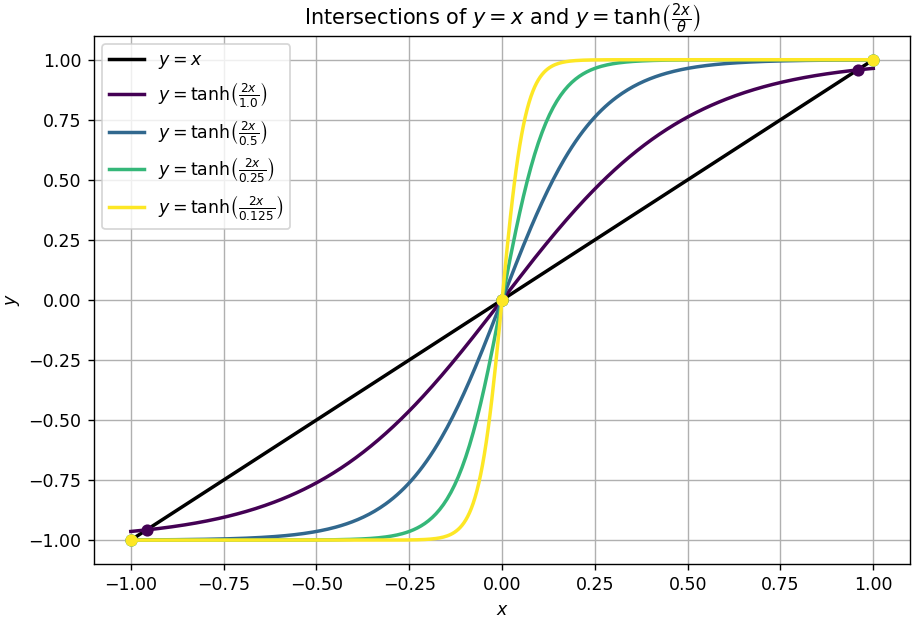
\includegraphics[width=1\linewidth]{Project plots/tanhthetav2.png}
       \vspace{-0.4cm}
    \caption{Intersections of $y = x$ and $y = \tanh\!\left(\frac{2x}{\theta}\right)$}
\end{figure}\FloatBarrier
\noindent From Figure 6 we see that as $\theta \to 0^+$, (the deep quench limit), $L_{y_0}(\theta) \to \pm 1$ for $y_0 \neq 0$. Since $f(y) \to \mp\infty$ as $y \to \pm 1$, it holds that for any fixed $\theta>0, \, T> 0$, it is possible to find $\delta t \ll 1 $  such that  $|y^{n+1}| = |y^n+\delta t f(y^n)| < 1\, \forall n\in \{0,1,2,\dots \frac{T}{\delta t} \}$. However, we can observe below on Figure 7 that as $\theta$ decreases, the maximum viable $\delta t$ to remain within the domain $(-1,1)$ decays towards $0$ very quickly. Therefore to numerically approximate solutions to this ODE for small values of $\theta$, we would require numerical precision to a level which will become unfeasible due to floating point limitations.  
\begin{figure}[!htb]
    \centering
    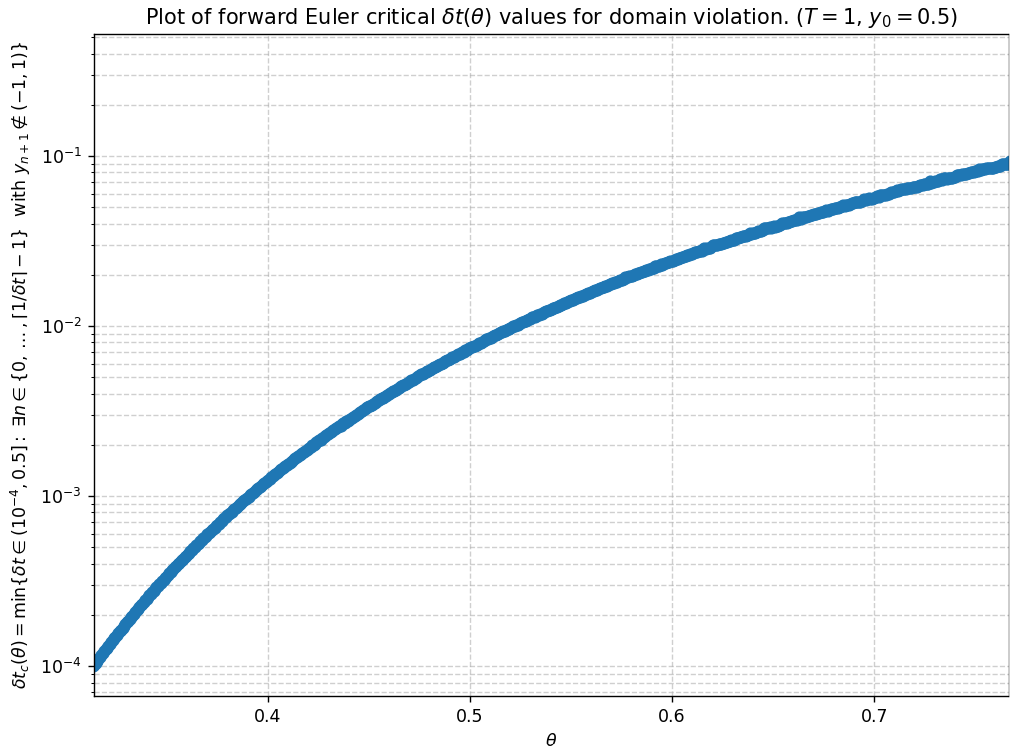
\includegraphics[width=1\linewidth]{Project plots/FE plot rescaled v2.1.png}
    \caption{Log scale plot of forward Euler critical $\delta t(\theta)$ values for domain violation. ($T=1$, $y_0=0.5$) - ($\theta \in (0.31,0.76)$, $\delta t \in (10^{-4},0.5)$). Source code in Appendix B.}
\end{figure} \FloatBarrier

\begin{enumerate}
    \setcounter{enumi}{6}
  \item Provide an implicit scheme to approximate the ODE.
  \end{enumerate}
  
  \noindent \textbf{SOLUTION:} \newline

    \noindent The implicit (backward Euler) scheme to approximate the ODE is:
    \[
    y^n = y^{n-1} + h_nf(t_n,y^n)
    \]
    So we have:
    \begin{align*}
        y^n &=y^{n-1} + h_n\left[ -\frac{\theta}{2}\left(\log(1+y^n)-\log(1-y^n)\right)+2y^n\right]\\
         &= y^{n-1} -\frac{\theta h_n}{2}\left(\log(1+y^n)-\log(1-y^n)\right)+2h_ny^n\\
         &= y^{n-1}-\frac{\theta h_n}{2} \log\left(\dfrac{1+y^n}{1-y^n}\right)+2h_ny^n\\
         \implies y^n-2h_ny^n &= y^{n-1}-\frac{\theta h_n}{2} \log\left(\dfrac{1+y^n}{1-y^n}\right)\\
         \implies y^n(1-2h_n)  &= y^{n-1}-\frac{\theta h_n}{2} \log\left(\dfrac{1+y^n}{1-y^n}\right)\\[5pt]
         \implies &\begin{cases}
             y^n  &= \dfrac{y^{n-1}-\dfrac{\theta h_n}{2} \log\left(\dfrac{1+y^n}{1-y^n}\right)}{(1-2h_n)} \quad;\quad n=1,2,\dots\\
             y^0 &= y_0\\[5pt]
         \end{cases}
    \end{align*}
\begin{enumerate}
    \setcounter{enumi}{7}
  \item State the non-linear problem which must be solved in the implicit scheme.
\end{enumerate}

  \noindent \textbf{SOLUTION:} \newline

\noindent The non-linear problem which must be solved under the implicit (backward Euler scheme) is given by the function $G:(-1,1)\to \mathbb{R}$ defined as:
\begin{align*}
    G(y) := \,& y- h_n\left[ -\frac{\theta}{2}\left(\log(1+y)-\log(1-y)\right)+2y\right]  - y^{n-1}\\[5pt]
    =\,& y - h_nf(y) - y^{n-1}
\end{align*}

\noindent Where $h_n, \theta, y^{n-1}$ are known, and given $y^{n-1} \in (-1,1)$ we need to find a solution, $y \in(-1,1)$ to:
\[
G(y) =0
\]
Whereby our solution to this non-linear problem, $y$, is $y^n$ which is then used in the next iteration to determine $y^{n+1}$. \newline

\noindent\textbf{Tough extension:}
\begin{itemize}
  \item Provide (pesudo-)code on how one might attempt to solve the implicit scheme this on a computer.
    \item Solve the ODE using your implicit scheme for $\theta = 1$.
  \item Solve the ODE using your implicit scheme for $\theta = 0.25$. \textbf{This is not for the faint
  of heart.} You may encounter troubles based on how you chose to ``solve this on a computer''.
  It may be beneficial to make use of the projection
  \[
    s \mapsto \max(\min(s,1-\varepsilon),-1+\varepsilon)
  \]
  for some very small $\varepsilon > 0$ at some point, if required.\\
  \end{itemize}
  \vspace{-0.3cm}
  \noindent \textbf{SOLUTION:} \newline

\noindent We will do all three of these extension questions together. We first apply Newton's method to find the roots of $G$ at each step $n$. We have:
\begin{align*}
    G(y) &= y - h_nf(y) - y^{n-1}\\[10pt]
    \implies G'(y) &= 1 - h_nf'(y)\\[4pt]
    &= 1 - h_n\left[ \frac{d}{dy}\left( -\frac{\theta}{2}\left(\log(1+y)-\log(1-y)\right)+2y \right) \right]\\[4pt]
    &= 1- h_n\left[ -\dfrac{\theta}{2}\left( \dfrac{1}{1+y} +\dfrac{1}{1-y}\right) + 2\right]
\end{align*}

\noindent Therefore our Newton's method to find $y^{n}$ at time step $n$, given we apply an initial guess of $y_{k=0} = y^{n-1}$, is:
\begin{align*}
y_{k+1} &= y_k - \frac{G(y_k)}{G'(y_k)}\,;\, k = 0,1,2,\dots K\\[3pt]
   &= y_k - \dfrac{y_k- h_n\left[ -\dfrac{\theta}{2}\left(\log(1+y_k)-\log(1-y_k)\right)+2y_k\right]  - y^{n-1}}{1- h_n\left[ -\dfrac{\theta}{2}\left( \dfrac{1}{1+y_k} +\dfrac{1}{1-y_k}\right) + 2\right]}\\[5pt]
    &= y_k - \dfrac{y_k-h_nf(y_k)-y^{n-1}}{1-h_nf'(y_k)}\\
\end{align*}
\noindent Taking increasing values of $K$, (assuming the iteration converges) we will have:
\[\displaystyle \lim_{K\to\infty} y_K = y^n\]

We can implement this in Python whereby we will:\newline
\begin{enumerate}
    \item Allow for solutions to be determined given:
    \begin{itemize}
        \item  Any initial condition: $y_0$\\
        \item  Any maximum time interval: $T$\\
        \item Any value of $\theta > 0$\\
        \item Any step size $h > 0$. (Where $h = \frac{T}{N}$).\\
        \item Any iteration count, $K$, the Newton method is applied over (set to $75$).\\
    \end{itemize}
    \item Plot the convergence of solutions to the steady states for $\theta =1 , 0.25$. \\
    \item Apply a piecewise projection $s \mapsto \max(\min(s,1-\epsilon),\epsilon-1)= 
\begin{cases} 
\epsilon - 1 & \text{if } s \leq \epsilon - 1 \\[3pt]
s & \text{if } \epsilon - 1 < s \leq 1 - \epsilon \\[3pt]
1 - \epsilon & \text{if } s > 1 - \epsilon\\[3pt]
\end{cases}$ to $y$ in each iteration of the Newton method (see line $22$) to ensure each $y_k$ remains on the domain $(-1,1)$ should the value of $\delta t = h$ used be too large (see figure 7).
\end{enumerate}
\[\]
\begin{minted}[linenos]{python}
import numpy as np; import matplotlib.pyplot as plt

class Config:
    y0_values = [-0.5, 0.0, 0.5]
    T = 2.0
    theta_values = [0.25, 1]
    h=1e-4
    K = 75
    epsilon = 1e-10
    
CFG = Config()
y0_values = CFG.y0_values; T = CFG.T; theta_values = CFG.theta_values; h = CFG.h; K = CFG.K
epsilon = CFG.epsilon; N = int(np.ceil(T / h))

def f(y, theta): return -0.5*theta*(np.log(1.0 + y) - np.log(1.0 - y)) + 2.0*y

def fdash(y, theta): return -0.5*theta*(1.0/(1.0 + y) + 1.0/(1.0 - y)) + 2.0

def Newton(y_prev, h, theta, K, epsilon):
    y = y_prev
    for k in range(K):
        y = np.clip(y, -1.0 + epsilon, 1.0 - epsilon)
        G = y - h * f(y, theta) - y_prev
        Gdash = 1.0 - h * fdash(y, theta)
        if Gdash == 0.0:
           break
        y = y - G / Gdash
    return y

def BE(theta, y0, T, h, K, epsilon):
    t = np.linspace(0.0, T, N + 1)
    y = np.empty(N + 1)
    y[0] = y0
    for n in range(1, N + 1):
        y[n] = Newton(y[n - 1], h, theta, K, epsilon)
    return t, y

for y0 in y0_values:
    plt.figure()
    for theta in theta_values:
        t, y = BE(theta, y0, T, h, K, epsilon)
        print(fr"Given: $y_0={y0}$, $T={T}$, $\theta={theta}$, $h = {h}$, $K={K}$, \
                $\epsilon={epsilon}$:")
        for i in [T * 0.0/5, T*1.0/5, T*2.0/5, T*3.0/5, T*4.0/5, T*5.0/5]:
            print(fr"$y({i}) =  {y[int(round(i / h))]:.12f}$")
        plt.plot(t, y, label=fr"$\theta = {theta}$")
        if theta == 1:
            plt.axhline(0.95750402*np.sign(y0), 
                        label=fr"Solution to explicit scheme with $\theta={theta}$",
                        color='green', linestyle='--', linewidth=0.8, zorder=2)
        if theta == 0.25:
            plt.axhline(0.999999774929*np.sign(y0), 
                        label=fr"Solution to explicit scheme with $\theta={theta}$",
                        color='red', linestyle='--', linewidth=0.8, zorder=2)
    plt.xlabel("t")
    plt.ylabel("y(t)")  
    plt.title(fr"Backward Euler solution of IVP ($y_0$ = {y0}, $T$ = {T},"
              fr"$\theta \in$ {{{ ", ".join(map(str, theta_values))}}}, "
              fr"$h$ = {h}, $K$ = {K}, $\epsilon$ = {epsilon})")     
    plt.legend(loc='lower right' if np.sign(y0) > 0 \
                                 else ('upper right' if np.sign(y0) < 0 else 'best'))
    plt.grid(True)
    plt.xlim(0, T)
    plt.ylim((0, 1+0.1) if np.sign(y0) > 0 \
                        else ((-0.1, 0.1) if np.sign(y0) == 0 else (-1-0.1, 0)))
    plt.show()
    \end{minted}
\[\]
\noindent Based on the above script, we get the following outputs on Tables $2$ and $3$ which are reflected in the plots on Figures $8,\,9,\,10$ respectively.\newline
\[\]
\begin{table}[H]
\centering
\caption{Backward Euler solutions to IVP for $t \in \{0,0.4,0.8,1.2,1.6,2.0\}$ given $T = 2.0$, $\theta = 0.25$, $h = 10^{-4}$, $K = 75$, $\epsilon = 10^{-10}$.}
\begin{tabular}{c|ccc}
\hline
    \diagbox[
      innerwidth=2em,
      height=1.8em,
      innerleftsep=0.3em,
      innerrightsep=0.3em
    ]{$t$}{$y_0$}
& $-0.5$ & $0$ & $0.5$ \\
\hline
0.0 & $-0.500000000000$ & $0.000000000000$ & $0.500000000000$ \\
0.4 & $-0.973824808972$ & $0.000000000000$ & $0.973824808972$ \\
0.8 & $-0.999999774929$ & $0.000000000000$ & $0.999999774929$ \\
1.2 & $-0.999999774929$ & $0.000000000000$ & $0.999999774929$ \\
1.6 & $-0.999999774929$ & $0.000000000000$ & $0.999999774929$ \\
2.0 & $-0.999999774929$ & $0.000000000000$ & $0.999999774929$ \\
\hline
\end{tabular}
\end{table}
\[\]
\begin{table}[H]
\centering
\caption{Backward Euler solutions to IVP for $t \in \{0,0.4,0.8,1.2,1.6,2.0\}$ given $T = 2.0$, $\theta = 1.0$, $h = 10^{-4}$, $K = 75$, $\epsilon = 10^{-10}$.}
\begin{tabular}{c|ccc}
\hline
    \diagbox[
      innerwidth=2em,
      height=1.8em,
      innerleftsep=0.3em,
      innerrightsep=0.3em
    ]{$t$}{$y_0$}
& $-0.5$ & $0$ & $0.5$ \\
\hline
0.0 & $-0.500000000000$ & $0.000000000000$ & $0.500000000000$ \\
0.4 & $-0.700268451297$ & $0.000000000000$ & $0.700268451297$ \\
0.8 & $-0.891838198267$ & $0.000000000000$ & $0.891838198267$ \\
1.2 & $-0.954740045037$ & $0.000000000000$ & $0.954740045037$ \\
1.6 & $-0.957451815615$ & $0.000000000000$ & $0.957451815615$ \\
2.0 & $-0.957503073361$ & $0.000000000000$ & $0.957503073361$ \\
\hline
\end{tabular}
\end{table}



\iffalse
\begin{table}[H]
\centering
\caption{Backward Euler solutions to IVP for $t \in \{0,0.4,0.8,1.2,1.6,2.0\}$ given $y_0 = -0.5$, $T = 2.0$, $\theta \in \{0.25, 1.0\}$, $h = 10^{-4}$, $K = 75$, $\epsilon = 10^{-10}$.}
\begin{tabular}{c|cc}
\hline
    \diagbox[
      innerwidth=2em,      
      height=1.6em,        
      innerleftsep=0.6em,  
      innerrightsep=0.6em  
    ]{$t$}{$\theta$}
& $0.25$ 
& $1.0$ \\
\hline
0.0 & $-0.500000000000$ & $-0.500000000000$ \\
0.4 & $-0.973824808972$ & $-0.700268451297$ \\
0.8 & $-0.999999774929$ & $-0.891838198267$ \\
1.2 & $-0.999999774929$ & $-0.954740045037$ \\
1.6 & $-0.999999774929$ & $-0.957451815615$ \\
2.0 & $-0.999999774929$ & $-0.957503073361$ \\
\hline
\end{tabular}
\end{table}


\begin{table}[H]
\centering
\caption{Backward Euler solutions to IVP for $t \in \{0,0.4,0.8,1.2,1.6,2.0\}$ given $y_0 = 0$, $T = 2.0$, $\theta \in \{0.25, 1.0\}$, $h = 10^{-4}$, $K = 75$, $\epsilon = 10^{-10}$.}
\begin{tabular}{c|cc}
\hline
    \diagbox[
      innerwidth=2em,      
      height=1.6em,        
      innerleftsep=0.6em,  
      innerrightsep=0.6em  
    ]{$t$}{$\theta$}
& $0.25$ 
& $1.0$ \\
\hline
0.0 & $0.000000000000$ & $0.000000000000$ \\
0.4 & $0.000000000000$ & $0.000000000000$ \\
0.8 & $0.000000000000$ & $0.000000000000$ \\
1.2 & $0.000000000000$ & $0.000000000000$ \\
1.6 & $0.000000000000$ & $0.000000000000$ \\
2.0 & $0.000000000000$ & $0.000000000000$ \\
\hline
\end{tabular}
\end{table}

\begin{table}[H]
\centering
\caption{Backward Euler solutions to IVP for $t \in \{0,0.4,0.8,1.2,1.6,2.0\}$ given $y_0 = 0.5$, $T = 2.0$, $\theta \in \{0.25, 1.0\}$, $h = 10^{-4}$, $K = 75$, $\epsilon = 10^{-10}$.}
\begin{tabular}{c|cc}
\hline
    \diagbox[
      innerwidth=2em,      
      height=1.6em,        
      innerleftsep=0.6em,  
      innerrightsep=0.6em  
    ]{$t$}{$\theta$}
& $0.25$ 
& $1.0$ \\
\hline
0.0 & $0.500000000000$ & $0.500000000000$ \\
0.4 & $0.973824808972$ & $0.700268451297$ \\
0.8 & $0.999999774929$ & $0.891838198267$ \\
1.2 & $0.999999774929$ & $0.954740045037$ \\
1.6 & $0.999999774929$ & $0.957451815615$ \\
2.0 & $0.999999774929$ & $0.957503073361$ \\
\hline
\end{tabular}
\end{table}
\fi



\begin{figure}[!htb]
    \centering
     \vspace{-0.1cm}
    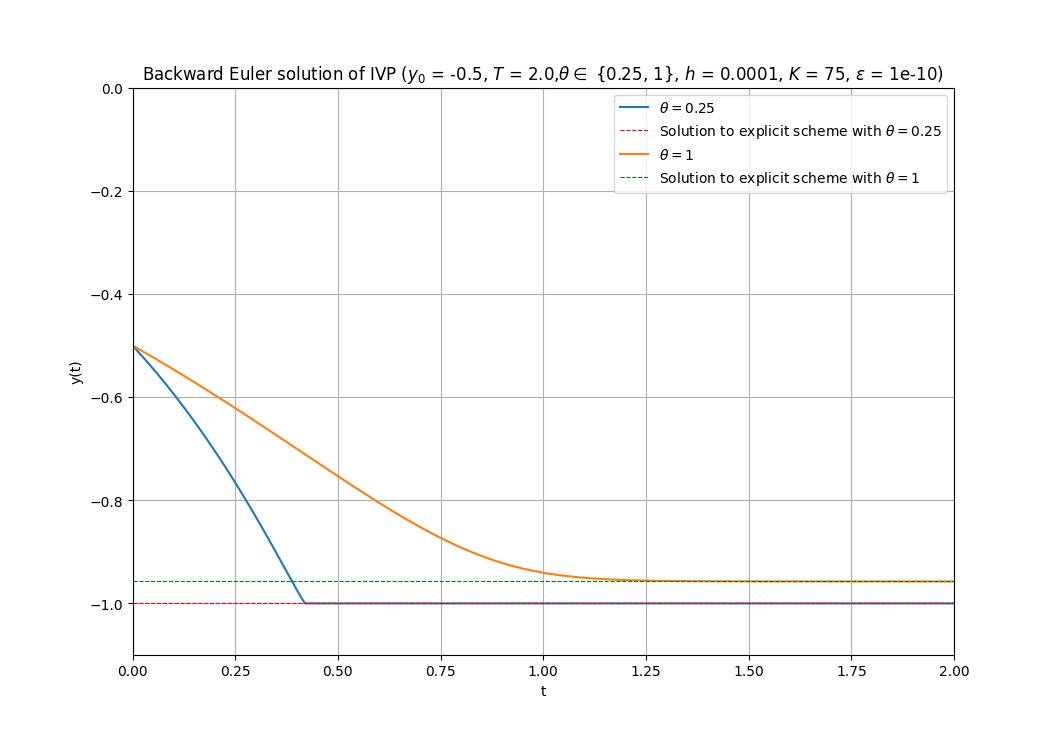
\includegraphics[width=1\linewidth]{Project plots/minus05.png}
  \vspace{-0.7cm}
    \caption{Backward Euler solution of IVP ($y_0 =-0.5$, $\theta \in \{0.25,1.0\}$)}
\end{figure}

\begin{figure}[!htb]
    \centering
  \vspace{0.3cm}
    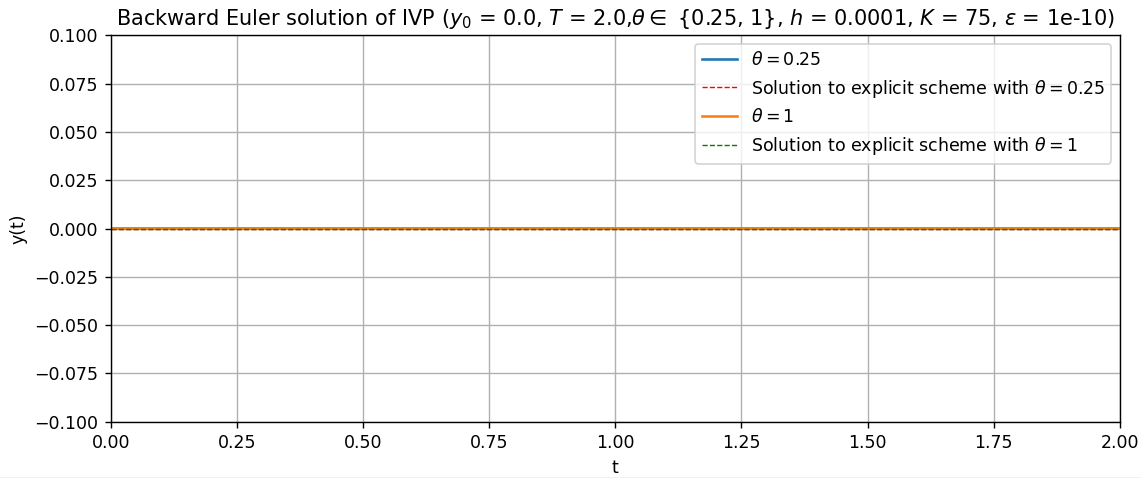
\includegraphics[width=1\linewidth]{Project plots/image.png}
        \vspace{-0.3cm}
    \caption{Backward Euler solution of IVP ($y_0 =0.0$, $\theta \in \{0.25,1.0\}$)}
\end{figure}

\begin{figure}[!htb]
    \centering
 \vspace{-0.3cm}
    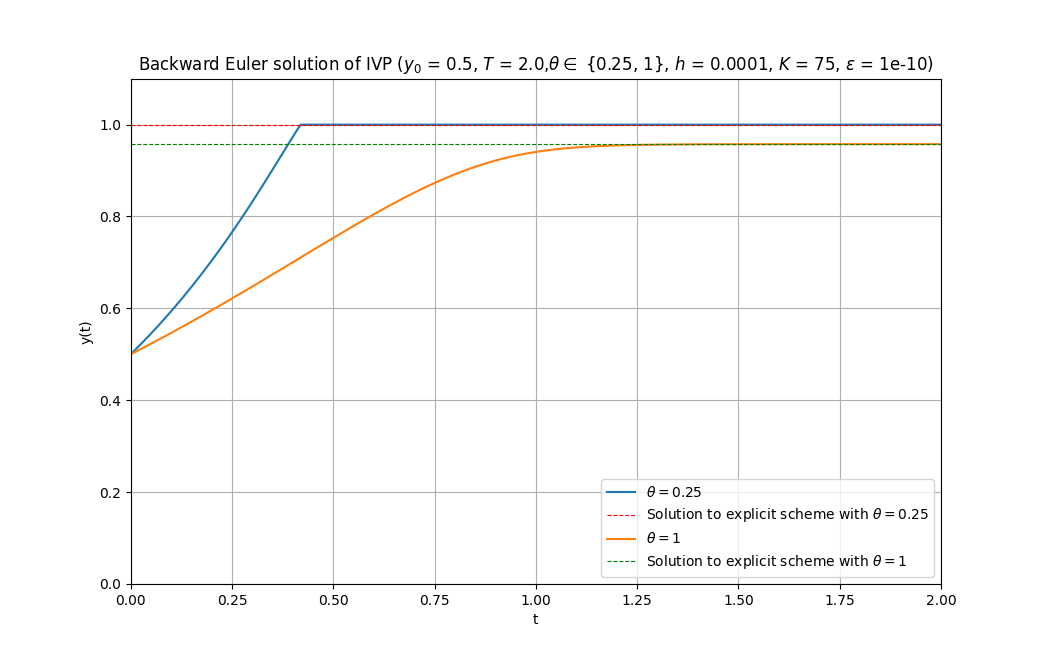
\includegraphics[width=1\linewidth]{Project plots/plus05.png}
     \vspace{-0.7cm}
    \caption{Backward Euler solution of IVP ($y_0 =0.5$, $\theta \in \{0.25,1.0\}$)}
\end{figure}\FloatBarrier
%\vspace{-1cm}
\newpage
\noindent \textbf{Appendix A - Forward Euler IVP solutions}
\begin{minted}[linenos]{python}
import numpy as np

class Config:
    theta = 1.0
    T = 1.0
    initial_conditions = [-0.5, 0.0, 0.5]
    dts = [0.1, 0.05, 0.025, 0.0125]
    epsilon = 1e-10
CFG = Config()
theta = CFG.theta; T = CFG.T; initial_conditions = CFG.initial_conditions
dts = CFG.dts; epsilon = CFG.epsilon

def f(y, theta):
    return -0.5 * theta * (np.log(1.0 + y) - np.log(1.0 - y)) + 2.0 * y

def FE(theta, y0, T, dt):
    N = int(round(T / dt))
    t = np.linspace(0.0, T, N + 1)
    y = np.empty(N + 1)
    y[0] = y0
    for n in range(N):
        y[n] = np.clip(y[n], -1.0 + epsilon, 1.0 - epsilon)
        y[n + 1] = y[n] + dt * f(y[n], theta)
    return t, y

for y0 in initial_conditions:
    for dt in dts:
        t, y = FE(theta, y0, T, dt)
        print(f"dt = {dt:.4f}, y0 = {y0}, y(1) = {y[-1]:.8f}")
\end{minted}
\newpage
\noindent \textbf{Appendix B - Critical $\delta t(\theta)$ plot}
\begin{minted}[linenos]{python}
import numpy as np
import matplotlib.pyplot as plt

class Config:
    y0 = 0.5
    T = 1.0
    min_theta = 0.3
    max_theta = 1.0
    number_thetas = 1000
    min_dt = 1e-4
    max_dt = 0.5
    grow=1.005
    
CFG = Config()
y0 = CFG.y0; T = CFG.T; min_theta = CFG.min_theta; max_theta = CFG.max_theta
number_thetas = CFG.number_thetas; min_dt = CFG.min_dt; max_dt = CFG.max_dt
grow = CFG.grow; theta_values = np.linspace(max_theta, min_theta, number_thetas)

def f(y, theta):
    return -0.5 * theta * (np.log(1.0 + y) - np.log(1.0 - y)) + 2.0 * y

def leaves_interval(y0, dt, T, theta):
    y = y0
    for i in range(int(np.ceil(T/dt))):
        y_new = y + dt * f(y, theta)
        if not (-1 < y_new < 1):
            return True
        y = y_new
    return False

def first_bad_dt(theta, y0, T, grow):
    dt = min_dt
    while dt <= max_dt:
        if leaves_interval(y0, dt, T, theta):
            return dt
        dt *= grow
    return None

critical = np.array([first_bad_dt(theta,y0,T, grow) for theta in theta_values], dtype=float)
plt.figure()
plt.plot(theta_values, critical, marker='o', linestyle='-')
plt.xlabel(r'$\theta$')
plt.ylabel(r'$\delta t_{c}(\theta) = \min\{\delta t\in(10^{-4},0.5]:\ \exists n\in '
           r'\{0,\dots,\lceil 1/\delta t\rceil-1\}\ \text{ with } y_{n+1}\notin(-1,1)\}$')
plt.title(r'Plot of forward Euler critical $\delta t(\theta)$ values for domain violation.'
          r' ($T=1$, $y_0=0.5$)')
plt.yscale('log')
plt.xlim(max_theta, min_theta)
plt.gca().invert_xaxis()
plt.grid(True, which='both', linestyle='--', alpha=0.6)
plt.tight_layout()
plt.show()
\end{minted}

\hrulefill


\end{document}


